\documentclass[11pt,letterpaper]{article}
\usepackage[utf8]{inputenc}
\usepackage[english]{babel}
\usepackage{latexsym,amsbsy,amssymb,amsmath,amsfonts}
\usepackage{amsthm}
\usepackage{epsfig}
\usepackage{euscript}
\usepackage{fullpage}
\usepackage{multirow,multicol,booktabs}
\usepackage[bf]{caption}
\usepackage{graphicx}
\usepackage{enumitem}
\usepackage{hyperref}
\hypersetup{
 pdfauthor={Christian Reitwießner},
 pdftitle={Babbage - a Mechanical Smart Contract Language}
  unicode,
  breaklinks,
  colorlinks=false,
  pdfborder={0 0 0}
}

\date{}

\renewcommand{\captionfont}{\small}


%%%%%%%%%%%%%%%%%%%%%%%%%%%%%%%%%%%%%%%%%%%%%%%%%%%%%%%%%%%%%
%%%%%%%%%%%%%%%%%%%%%%%%%%%%%%%%%%%%%%%%%%%%%%%%%%%%%%%%%%%%%
%%%%%%%%%%%%%%%%%%%%%%%%%%%%%%%%%%%%%%%%%%%%%%%%%%%%%%%%%%%%%


\hfuzz=0mm
\tolerance=10000
\hbadness=1000


\setlength{\parindent}{0mm}
\setlength{\parskip}{2ex plus0.5ex minus0.5ex}


\newcommand{\Sum}{\sum\limits}
\newcommand{\Prod}{\prod\limits}


\newtheorem{dummytheorem}{Dummy-Theorem}[section]
\newtheorem{definition}[dummytheorem]{Definition}
\newtheorem{lemma}[dummytheorem]{Lemma}
\newtheorem{theorem}[dummytheorem]{Theorem}
\newtheorem{proposition}[dummytheorem]{Proposition}
\newtheorem{property}[dummytheorem]{Property}
\newtheorem{corollary}[dummytheorem]{Corollary}
\newtheorem{example}[dummytheorem]{Example}
\newtheorem{remark}[dummytheorem]{Remark}
\newtheorem{fact}[dummytheorem]{Fact}
\newtheorem{claim}[dummytheorem]{Claim}
\newtheorem{subclaim}{Subclaim}[dummytheorem]
\newtheorem{conjecture}[dummytheorem]{Conjecture}

\newcommand{\uint}{\mathbb{N}}
\newcommand{\rational}{\mathbb{Q}}

\newcommand{\oli}[1]{\overline{#1}}

%%%%%%%%%%%%%%%%%%%%%%%%%%%%%%%%%%%%%%%%%%%%%%%%%%%%%%%%%%%%%%%%%%%%%%%%%%%%%%%%
%%%%%%%%%%%%%%%%%%%%%%%%%%%%%%%%%%%%%%%%%%%%%%%%%%%%%%%%%%%%%%%%%%%%%%%%%%%%%%%%
%%%%%%%%%%%%%%%%%%%%%%%%%%%%%%%%%%%%%%%%%%%%%%%%%%%%%%%%%%%%%%%%%%%%%%%%%%%%%%%%



\newcommand{\eps}{\varepsilon}
\newcommand{\card}[1]{\##1}
\newcommand{\length}[1]{\mathrm{length}({#1})}

\newcommand{\pn}[1]{\textnormal{#1}}

\newcommand{\norm}[1]{||{#1}||}
\newcommand{\Norm}[1]{\left|\left|{#1}\right|\right|}



%%%%%%%%%%%%%%%%%%%%%%%%%%%%%%%%%%%%%%%%%%%%%%%%%%%%%%%%%%%%%%%%%%%%%%%%%%%%%%%%
%%%%%%%%%%%%%%%%%%%%%%%%%%%%%%%%%%%%%%%%%%%%%%%%%%%%%%%%%%%%%%%%%%%%%%%%%%%%%%%%
%%%%%%%%%%%%%%%%%%%%%%%%%%%%%%%%%%%%%%%%%%%%%%%%%%%%%%%%%%%%%%%%%%%%%%%%%%%%%%%%


\begin{document}
\selectlanguage{english}


\title{Babbage -- a Mechanical Smart Contract Language}

\author{Christian Reitwießner\\
{\tt chris@ethereum.org}}


\maketitle


\begin{abstract}
\noindent Smart contract programming languages should be easy to understand
and unambiguous. Usually, such languages are written in formal computer languages
comprised of functions and variables. While this already makes them quite
abstract and hard to understand, the fact that components of a smart contract
can be referenced by name partly from anywhere in the program sometimes
makes it almost impossible to see how different parts interact and fit together.

We propose a language that is situated at a level even untrained people can
understand. Babbage is a visual programming language that consists of simple
mechanical parts that interact with each other: Rods, levers, cords, springs
and simple pneumatic hoses. Since components that want to interact with each
other have to be physically close, the modularity of such systems is already
guaranteed by design. Furthermore, people with no knowledge of programming
languages have the chance to understand complex smart contracts.
\end{abstract}

A smart contract on Ethereum can be described as a vending machine made of
glass, put at a public place:
Once it is created, it is not possible to modify it, except by pushing the buttons
that are mounted at its exterior. Furthermore, everyone has the possibility
to watch how it works internally. Note that open source software installed
on cloud computers is similar, but there is still an important difference:
You can take a look at the published source code, but you have no way to tell whether
the server actually runs the same code. This is similar to a vending machine
not made of glass: You can look at the blueprints, but you never know what
the machine actually does.

If the machine is made of glass, it is (depending on its complexity) quite
easy to see what will happen if you put a coin inside and then push a button.
You can even see if the drink you want to buy is still available.

We want to take this analogy further and build actual machines inside Ethereum.
The benefits are that humans should be able to figure out how a mechanical
machine works without any prior knowledge. Furthermore, it should be quite
easy to see any possible way in which a switch (a variable in text-based
programming languages) can be modified, because there has to be a physical
connection to that switch. Finally, as Ether is modeled as a liquid flowing
in pipes, you can directly see where it will go.

Also note that (software) engineers often resort to diagrams when they
want to explain something. Admittedly, diagrams often simplify things and
thus, a mechanical smart contract language might not be as expressive as
a text-based language, but on the other hand, mechanisms that are so complex
that they cannot be fully explained using a diagram should perhaps not be used
for smart contracts anyway.

Let's start with an example. A smart contract that distributes
all Ether sent to it equally among two addresses can be seen in Figure \ref{splitter}.
The dashed outer line delimits the smart contract. Anything that comes from
the environment or influences the environment has to extend towards the dashed line.
Ether is a purple liquid that flows in pipes which always have a flowing direction.
The smart contract has no way to store Ether, everything is just forwarded.
Ether comes in at the top, at the entry that is unmarked. The exits at the
bottom are marked and they are connected to these addresses and this connection
cannot be changed (there is no mechanism depicted that would be able to move the
pipes). The most interesting part of the smart contract is the splitter at the
middle. It has an indicator that tells how much of the input Ether goes to the
left exit and how much goes to the right exit. To help reading the indicator,
the exact percentages are also written in numbers.

\begin{figure}
\center
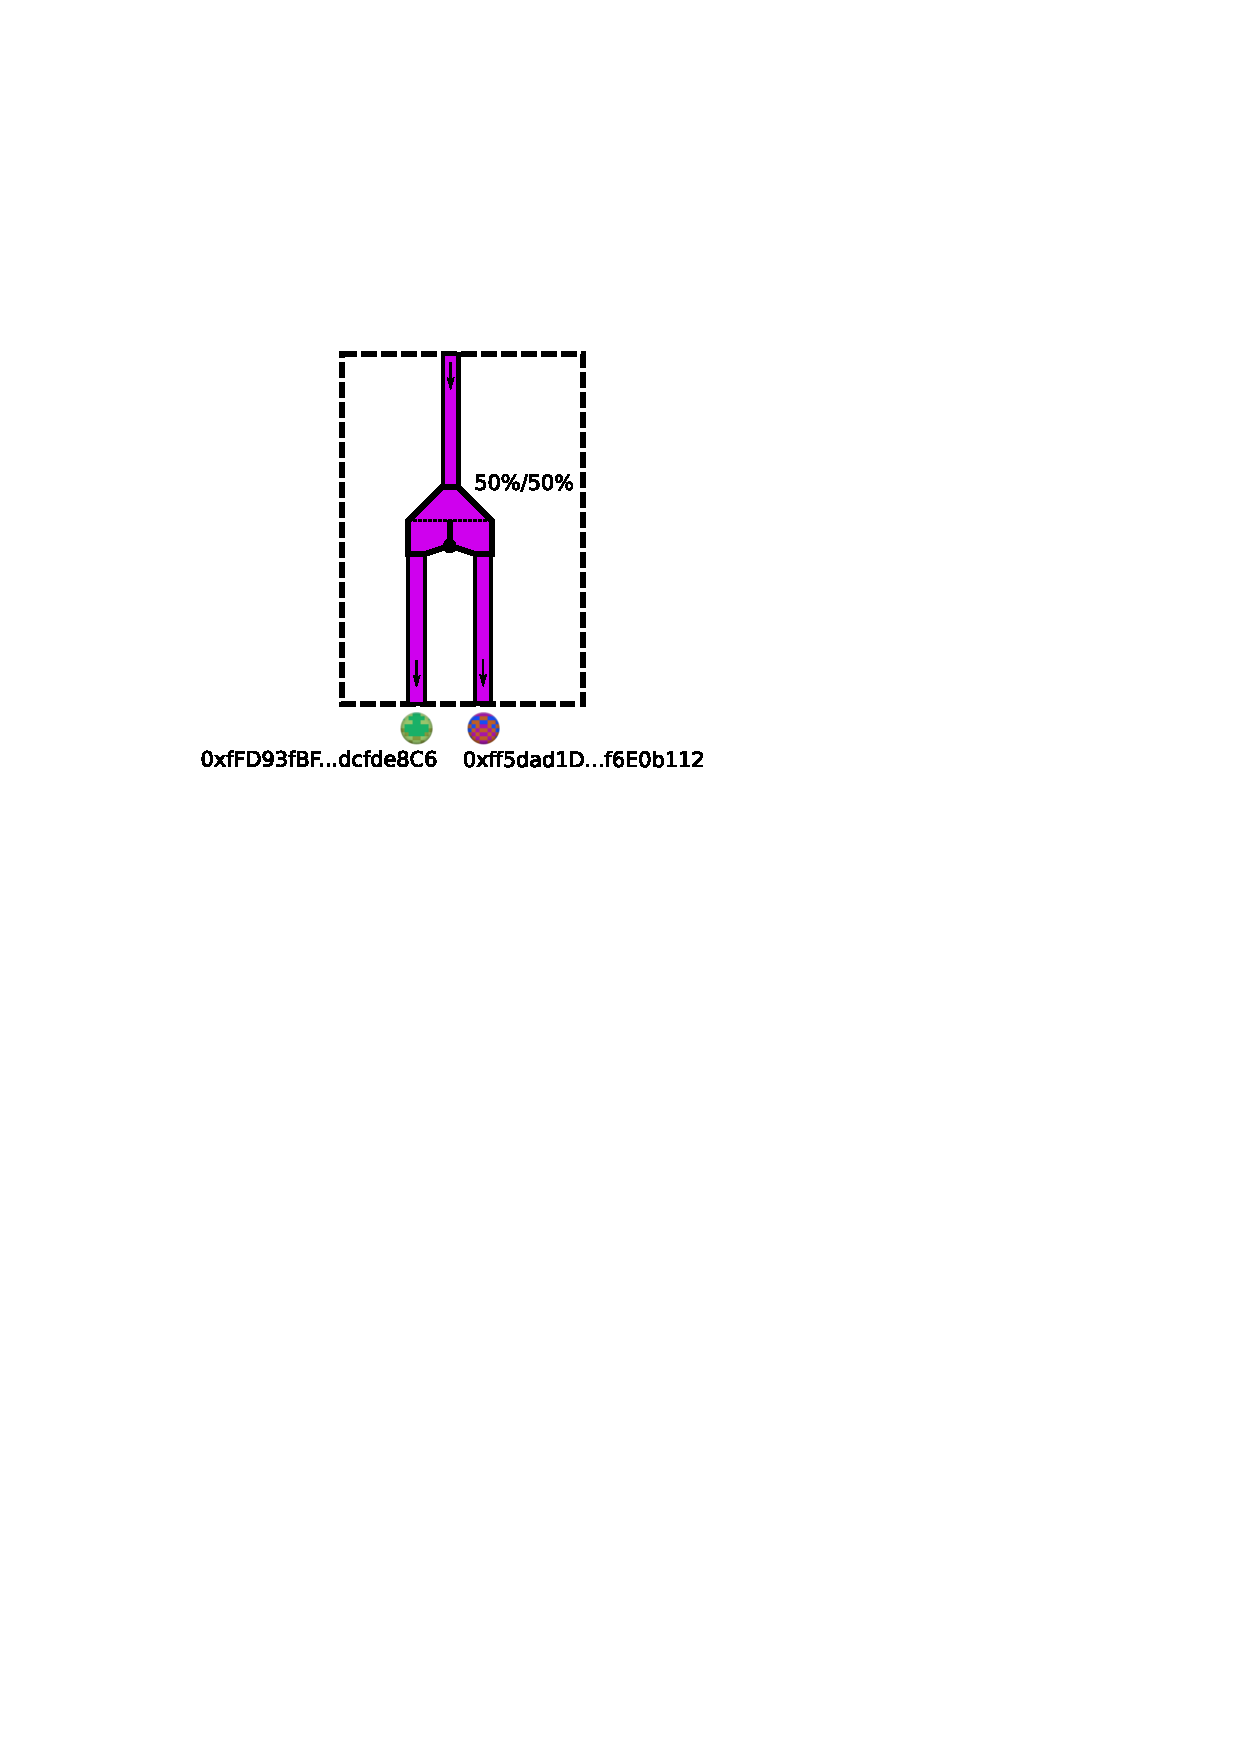
\includegraphics[height=4cm]{splitter.pdf}
\caption{Smart contract that distributes all Ether sent to it equally among
two addresses.}
\label{splitter}
\end{figure}

Let us now look at an extension of this simple splitter, the adjustable splitter,
which can be seen in Figure \ref{adjustable_splitter}.
This contract has a small button or lever at the outside and an address
written next to it telling that only this address is allowed to manipulate the
button.

\begin{figure}
\center
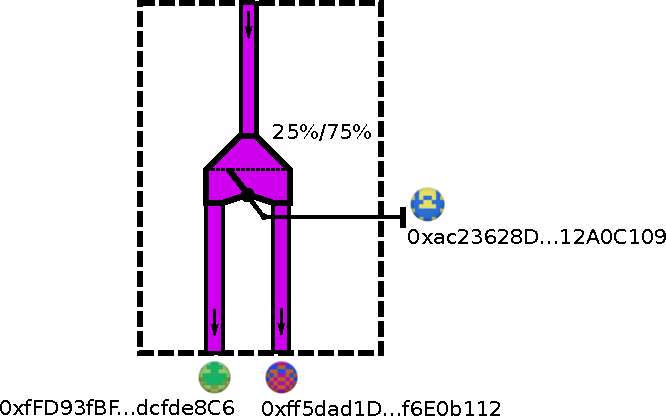
\includegraphics[height=4cm]{adjustable_splitter.pdf}
\caption{Smart contract that distributes all Ether sent to it among
two addresses with a ratio modifiable from a certain address.}
\label{adjustable_splitter}
\end{figure}

The last example shows another extension of the basic example. In Figure
\ref{multisig_splitter}, you can see a similar splitter whose ratio is controlled
by a two-of-three multisig mechanism.

\end{document}
